\begin{figure}[h]
\begin{center}
\beginpgfgraphicnamed{plot_ACCvsEntry.pdf}
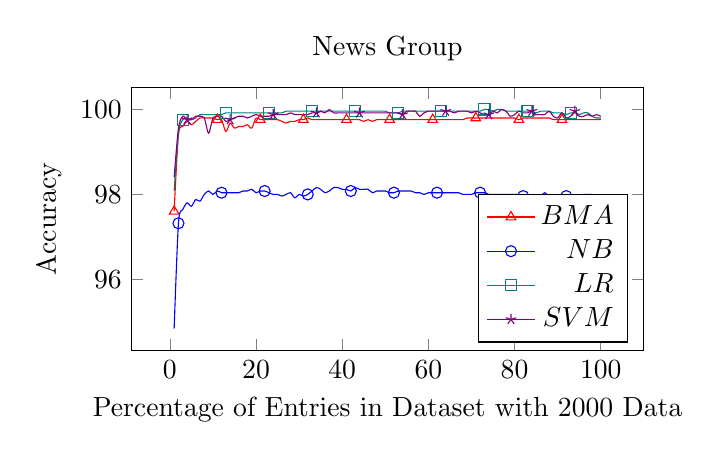
\begin{tikzpicture}
\begin{axis}
[title=News Group,
%ymin=0.5,
ylabel=Accuracy,
xlabel=Percentage of Entries in Dataset with 2000 Data,
%cycle list name=color list,
cycle list={%
    red,blue,teal,violet,cyan,green!70!black,magenta,gray},
width=230pt,
height=140pt,
legend style={
	cells = {anchor = east},
	legend pos = south east,
	},
]
\addplot+[smooth, mark=triangle, mark repeat=10,mark phase=1] coordinates
%\addplot coordinates
        {(1,97.6000) (2,99.4000) (3,99.6000) (4,99.7200) (5,99.6400) (6,99.7200) (7,99.8000) (8,99.8000) (9,99.8000) (10,99.8000) (11,99.7600) (12,99.7600) (13,99.4800) (14,99.6800) (15,99.5600) (16,99.6000) (17,99.6000) (18,99.6400) (19,99.5600) (20,99.8000) (21,99.7600) (22,99.7600) (23,99.7600) (24,99.7600) (25,99.7600) (26,99.7200) (27,99.6800) (28,99.7200) (29,99.7200) (30,99.7600) (31,99.7600) (32,99.8000) (33,99.7600) (34,99.7600) (35,99.7600) (36,99.7600) (37,99.7600) (38,99.7600) (39,99.7600) (40,99.7600) (41,99.7600) (42,99.7600) (43,99.7600) (44,99.7600) (45,99.7200) (46,99.7600) (47,99.7200) (48,99.7600) (49,99.7600) (50,99.7600) (51,99.7600) (52,99.7600) (53,99.7600) (54,99.7600) (55,99.7600) (56,99.7600) (57,99.7600) (58,99.7600) (59,99.7600) (60,99.7600) (61,99.7600) (62,99.7600) (63,99.7600) (64,99.7600) (65,99.7600) (66,99.7600) (67,99.7600) (68,99.7600) (69,99.8000) (70,99.8000) (71,99.8000) (72,99.8000) (73,99.8000) (74,99.8000) (75,99.8000) (76,99.8000) (77,99.8000) (78,99.8000) (79,99.8000) (80,99.8000) (81,99.7600) (82,99.8000) (83,99.8000) (84,99.8000) (85,99.8000) (86,99.8000) (87,99.8000) (88,99.8000) (89,99.7600) (90,99.7600) (91,99.7600) (92,99.7600) (93,99.7600) (94,99.7600) (95,99.7600) (96,99.7600) (97,99.7600) (98,99.7600) (99,99.7600) (100,99.7600)};
\addplot+[smooth,mark=o,  mark repeat=10,mark phase=2] coordinates
%\addplot coordinates
        {(1,94.8400) (2,97.3200) (3,97.6400) (4,97.8000) (5,97.7200) (6,97.8800) (7,97.8400) (8,98.0000) (9,98.0800) (10,98.0000) (11,98.0800) (12,98.0400) (13,98.0400) (14,98.0400) (15,98.0400) (16,98.0400) (17,98.0800) (18,98.0800) (19,98.1200) (20,98.0400) (21,98.0800) (22,98.0800) (23,98.0400) (24,98.0000) (25,98.0000) (26,97.9600) (27,98.0000) (28,98.0400) (29,97.9200) (30,98.0000) (31,97.9600) (32,98.0000) (33,98.0800) (34,98.1600) (35,98.1200) (36,98.0400) (37,98.0800) (38,98.1600) (39,98.1600) (40,98.1200) (41,98.1200) (42,98.0800) (43,98.1600) (44,98.1200) (45,98.1200) (46,98.1200) (47,98.0400) (48,98.0800) (49,98.0800) (50,98.0800) (51,98.0400) (52,98.0400) (53,98.0800) (54,98.0800) (55,98.0800) (56,98.0800) (57,98.0400) (58,98.0400) (59,98.0000) (60,98.0400) (61,98.0400) (62,98.0400) (63,98.0400) (64,98.0400) (65,98.0400) (66,98.0400) (67,98.0400) (68,98.0000) (69,98.0000) (70,98.0000) (71,98.0400) (72,98.0400) (73,98.0400) (74,98.0000) (75,98.0000) (76,98.0000) (77,98.0000) (78,98.0000) (79,98.0000) (80,98.0000) (81,98.0000) (82,97.9600) (83,97.9600) (84,97.9600) (85,97.9600) (86,97.9600) (87,98.0400) (88,97.9600) (89,97.9600) (90,97.9600) (91,98.0000) (92,97.9600) (93,98.0000) (94,97.9600) (95,97.9600) (96,98.0000) (97,98.0000) (98,98.0000) (99,97.9600) (100,98.0000) };
\addplot+[smooth,mark=square, mark repeat=10,mark phase=3] coordinates
%\addplot coordinates
{(1,98.0800) (2,99.4400) (3,99.7600) (4,99.8000) (5,99.7600) (6,99.8000) (7,99.8800) (8,99.8800) (9,99.8800) (10,99.8800) (11,99.8800) (12,99.8800) (13,99.9200) (14,99.9200) (15,99.9200) (16,99.9200) (17,99.9200) (18,99.9200) (19,99.9200) (20,99.9200) (21,99.9200) (22,99.9200) (23,99.9200) (24,99.9200) (25,99.9200) (26,99.9200) (27,99.9600) (28,99.9600) (29,99.9600) (30,99.9600) (31,99.9600) (32,99.9600) (33,99.9600) (34,99.9600) (35,99.9600) (36,99.9600) (37,99.9600) (38,99.9600) (39,99.9600) (40,99.9600) (41,99.9600) (42,99.9600) (43,99.9600) (44,99.9600) (45,99.9600) (46,99.9600) (47,99.9600) (48,99.9600) (49,99.9600) (50,99.9600) (51,99.9200) (52,99.9200) (53,99.9200) (54,99.9600) (55,99.9600) (56,99.9600) (57,99.9600) (58,99.9600) (59,99.9600) (60,99.9600) (61,99.9600) (62,99.9600) (63,99.9600) (64,99.9600) (65,99.9600) (66,99.9600) (67,99.9600) (68,99.9600) (69,99.9600) (70,99.9600) (71,99.9600) (72,99.9600) (73,100.0000) (74,100.0000) (75,99.9600) (76,100.0000) (77,100.0000) (78,99.9600) (79,99.9600) (80,99.9600) (81,99.9600) (82,99.9600) (83,99.9600) (84,99.9600) (85,99.9200) (86,99.9600) (87,99.9600) (88,99.9600) (89,99.9200) (90,99.9200) (91,99.9200) (92,99.8800) (93,99.9200) (94,99.9200) (95,99.8800) (96,99.9200) (97,99.9200) (98,99.8400) (99,99.8000) (100,99.8000)};
\addplot+[smooth,mark=star, mark repeat=10,mark phase=4] coordinates
%\addplot coordinates
{(1,98.4000) (2,99.5600) (3,99.8400) (4,99.7600) (5,99.7600) (6,99.8400) (7,99.8400) (8,99.8000) (9,99.4400) (10,99.8000) (11,99.8400) (12,99.8400) (13,99.7200) (14,99.7600) (15,99.8000) (16,99.8400) (17,99.8400) (18,99.8000) (19,99.8400) (20,99.8800) (21,99.8400) (22,99.8400) (23,99.8400) (24,99.8800) (25,99.8800) (26,99.8800) (27,99.8800) (28,99.9200) (29,99.8800) (30,99.8800) (31,99.8800) (32,99.8800) (33,99.9200) (34,99.9200) (35,99.9600) (36,99.9200) (37,100.0000) (38,99.9200) (39,99.9200) (40,99.9200) (41,99.9200) (42,99.9200) (43,99.9200) (44,99.9200) (45,99.9200) (46,99.9200) (47,99.9200) (48,99.9200) (49,99.9200) (50,99.9200) (51,99.9200) (52,99.9200) (53,99.9200) (54,99.8800) (55,99.9600) (56,99.9600) (57,99.9600) (58,99.8400) (59,99.9200) (60,99.9600) (61,99.9600) (62,99.9600) (63,99.9600) (64,99.9600) (65,99.9600) (66,99.9200) (67,99.9600) (68,99.9600) (69,99.9600) (70,99.9200) (71,99.9600) (72,99.9200) (73,99.8800) (74,99.8800) (75,99.9600) (76,99.9200) (77,100.0000) (78,99.9600) (79,99.8400) (80,99.8800) (81,99.9600) (82,99.9200) (83,99.9200) (84,99.9600) (85,99.8800) (86,99.8800) (87,99.8800) (88,99.9600) (89,99.8400) (90,99.8000) (91,99.9200) (92,99.8000) (93,99.8400) (94,99.9600) (95,99.8400) (96,99.8400) (97,99.8800) (98,99.8400) (99,99.8800) (100,99.8400)};
\legend{$BMA$,$NB$,$LR$,$SVM$}
\end{axis}
\end{tikzpicture}
\endpgfgraphicnamed
\end{center}
\caption{Classification Accuracy VS Number of Entries in dataset}
\end{figure}